\section{Simulink Diagrams}\label{text:simulink}
\begin{figure}[h]
	\centering
		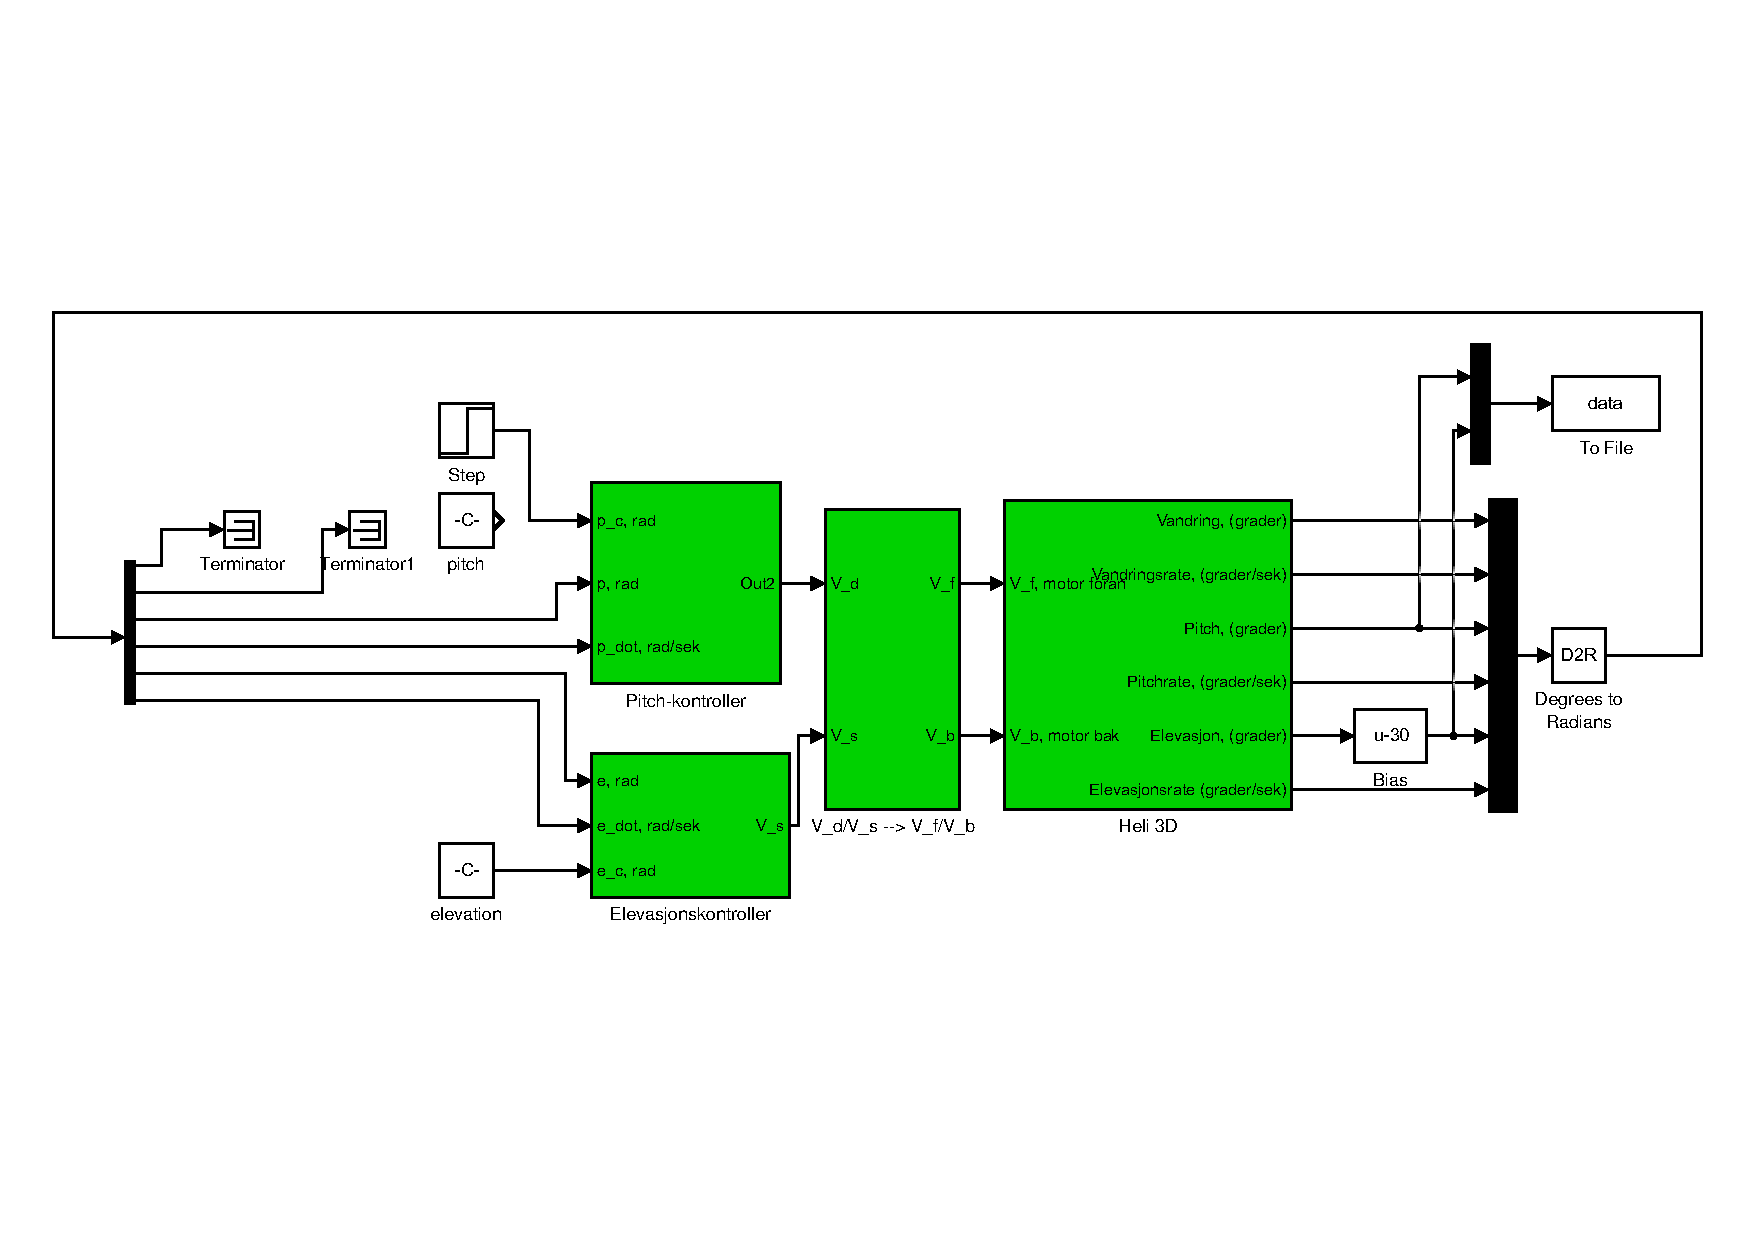
\includegraphics[width = 0.70\textwidth]{figures/1/simulink.pdf}
	\caption{Simulink model used in section \ref{text:problem1}.}
\end{figure}
\begin{figure}[h]
	\centering
		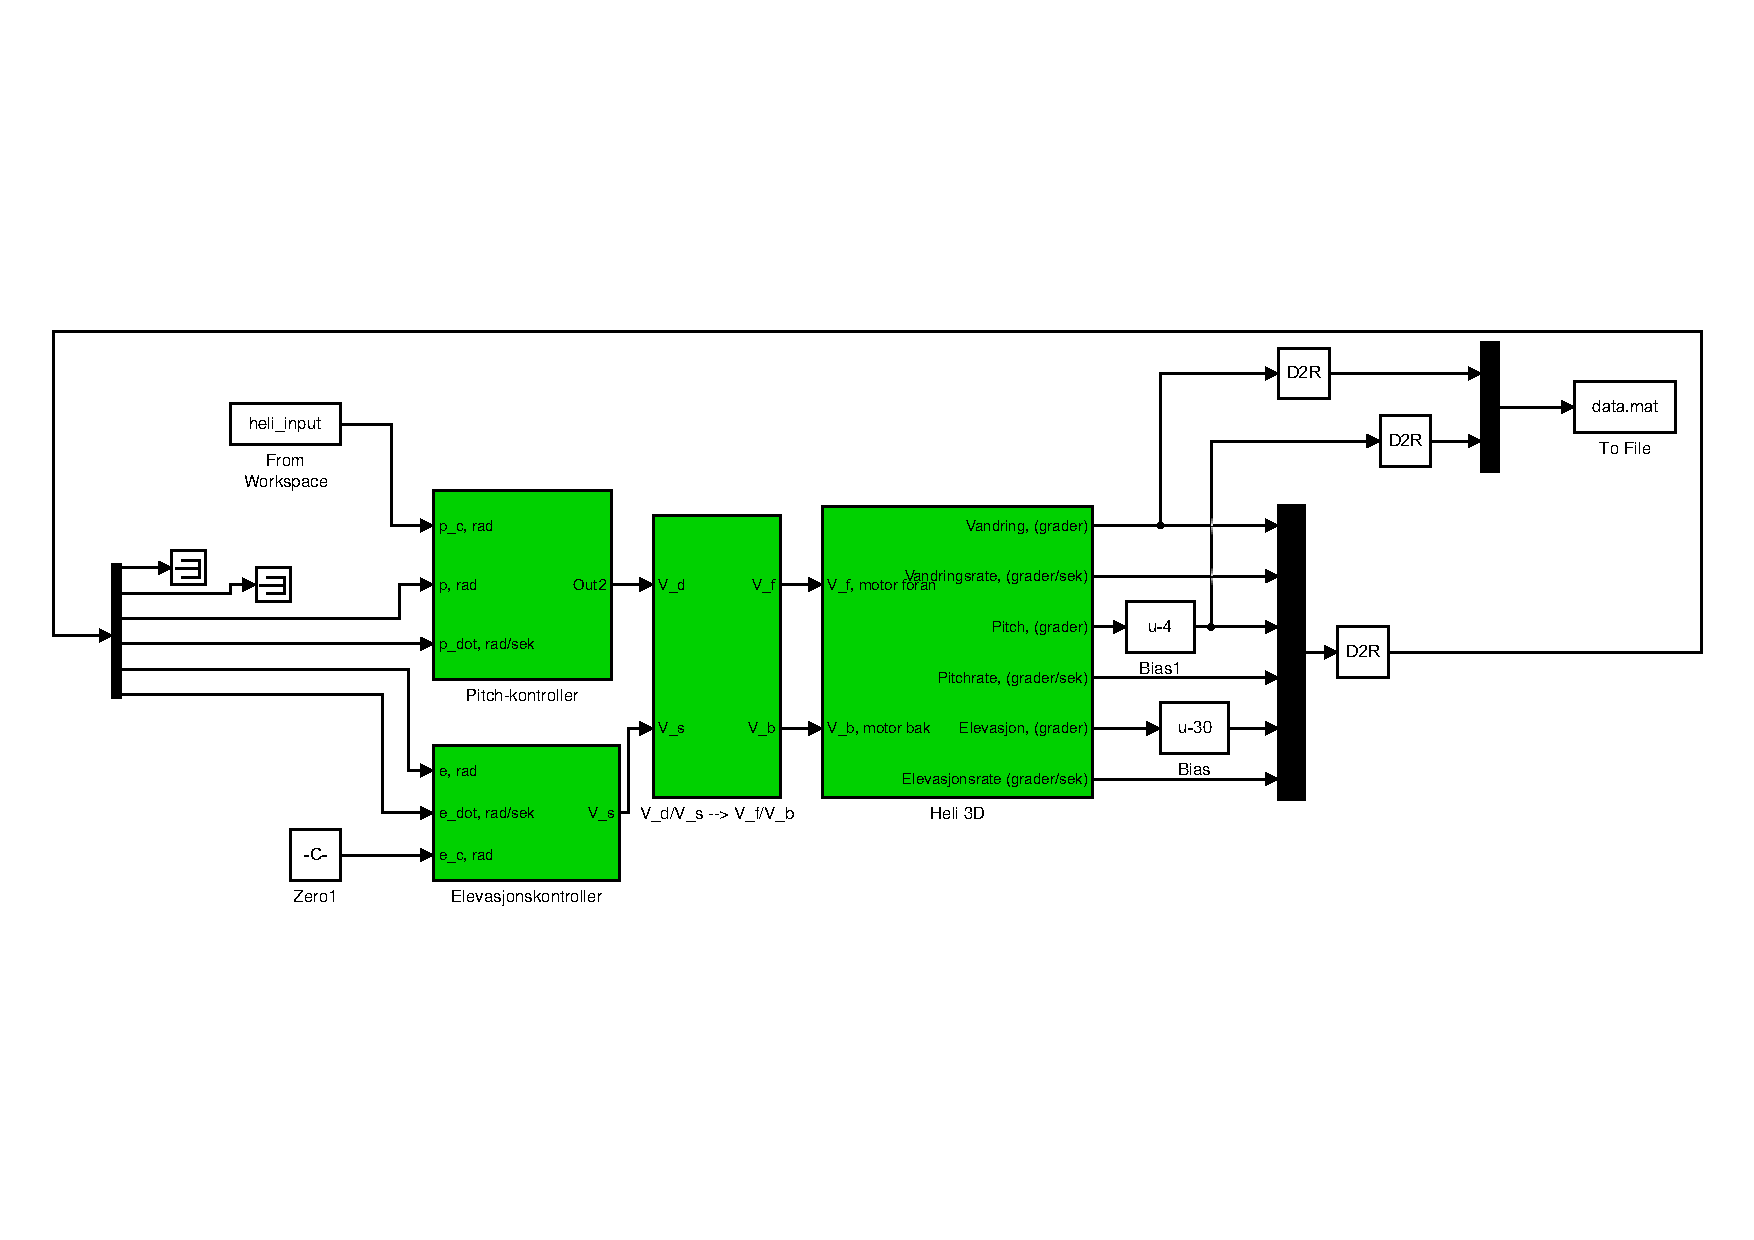
\includegraphics[width = 0.70\textwidth]{figures/2/simulink.pdf}
	\caption{Simulink model used in section \ref{text:problem2}.}
\end{figure}

\begin{figure}[h]
	\centering
		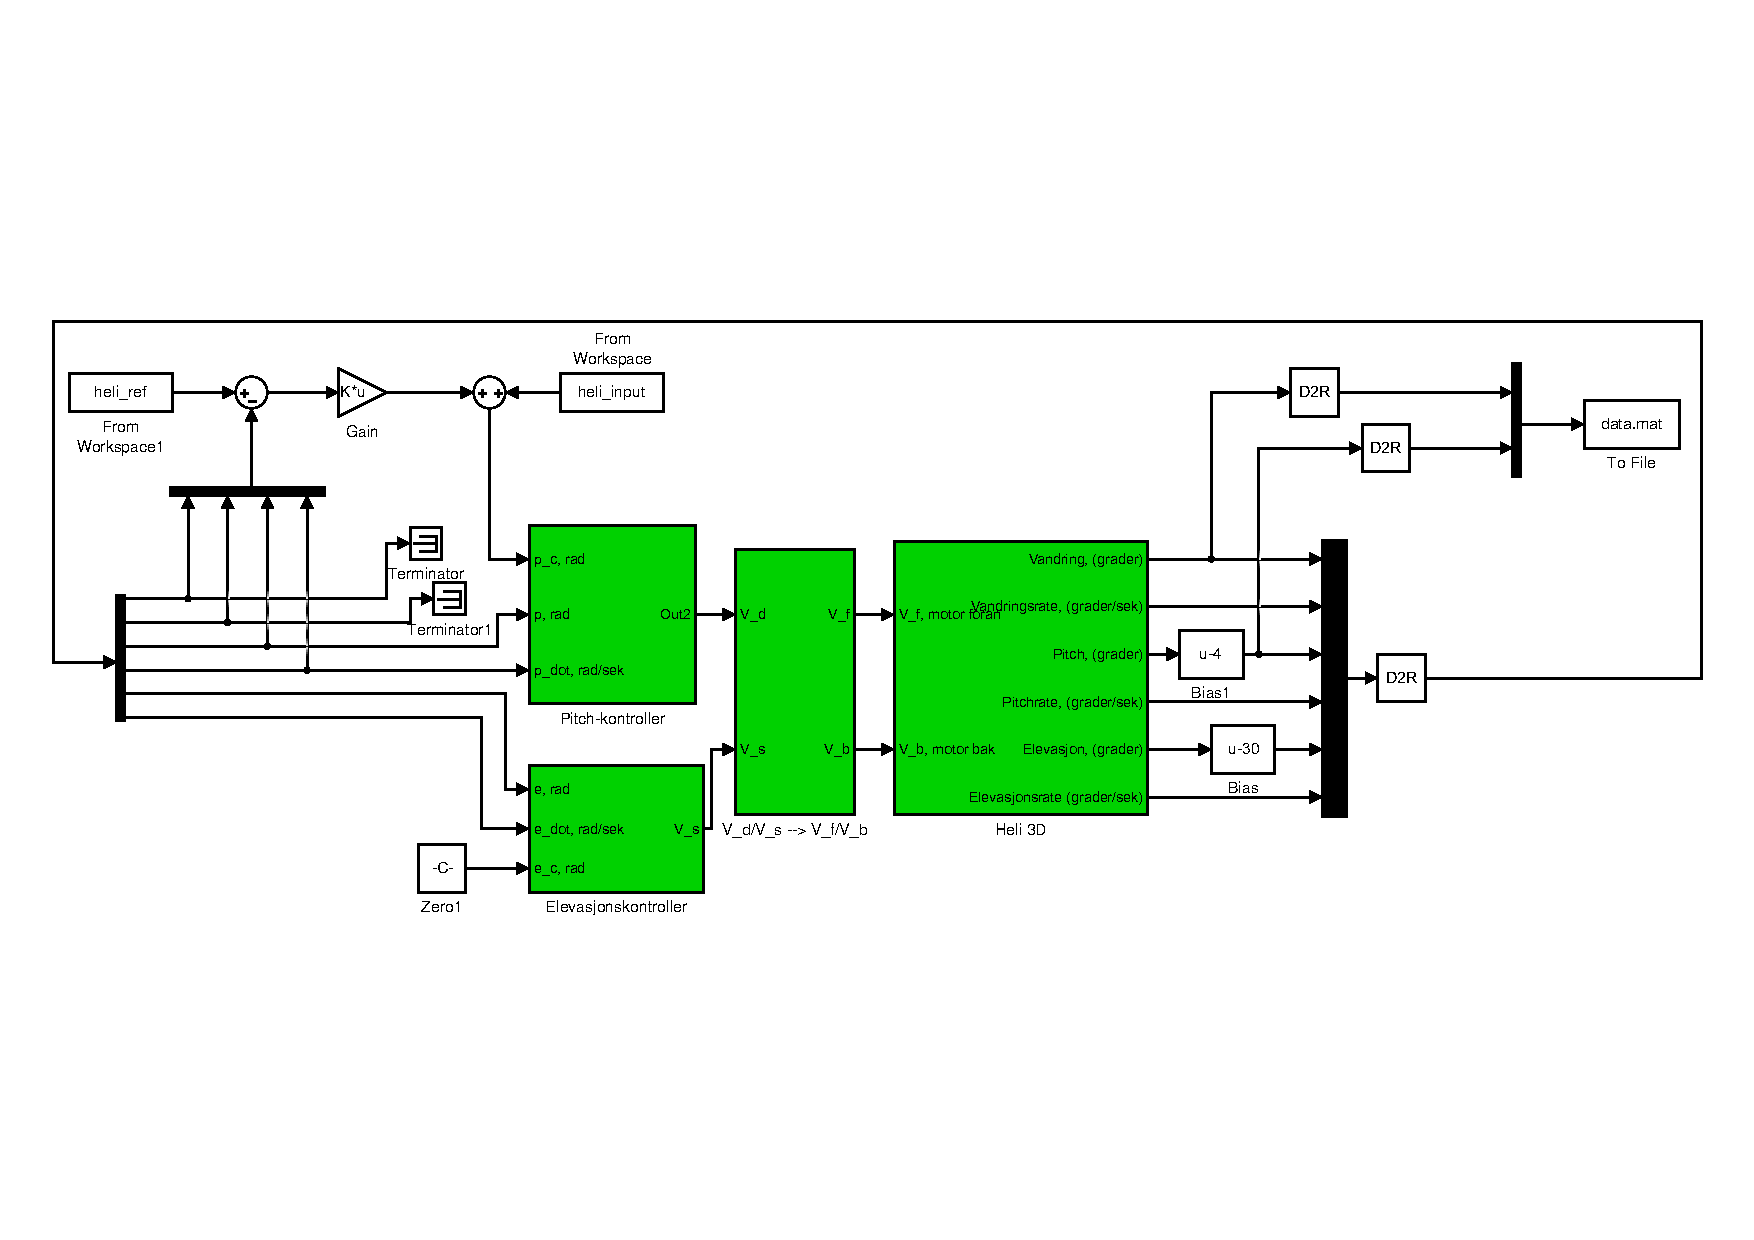
\includegraphics[width = 0.80\textwidth]{figures/3/simulink.pdf}
	\caption{Simulink model used in section \ref{text:problem3}.}
\end{figure}

\begin{figure}[h]
	\centering
		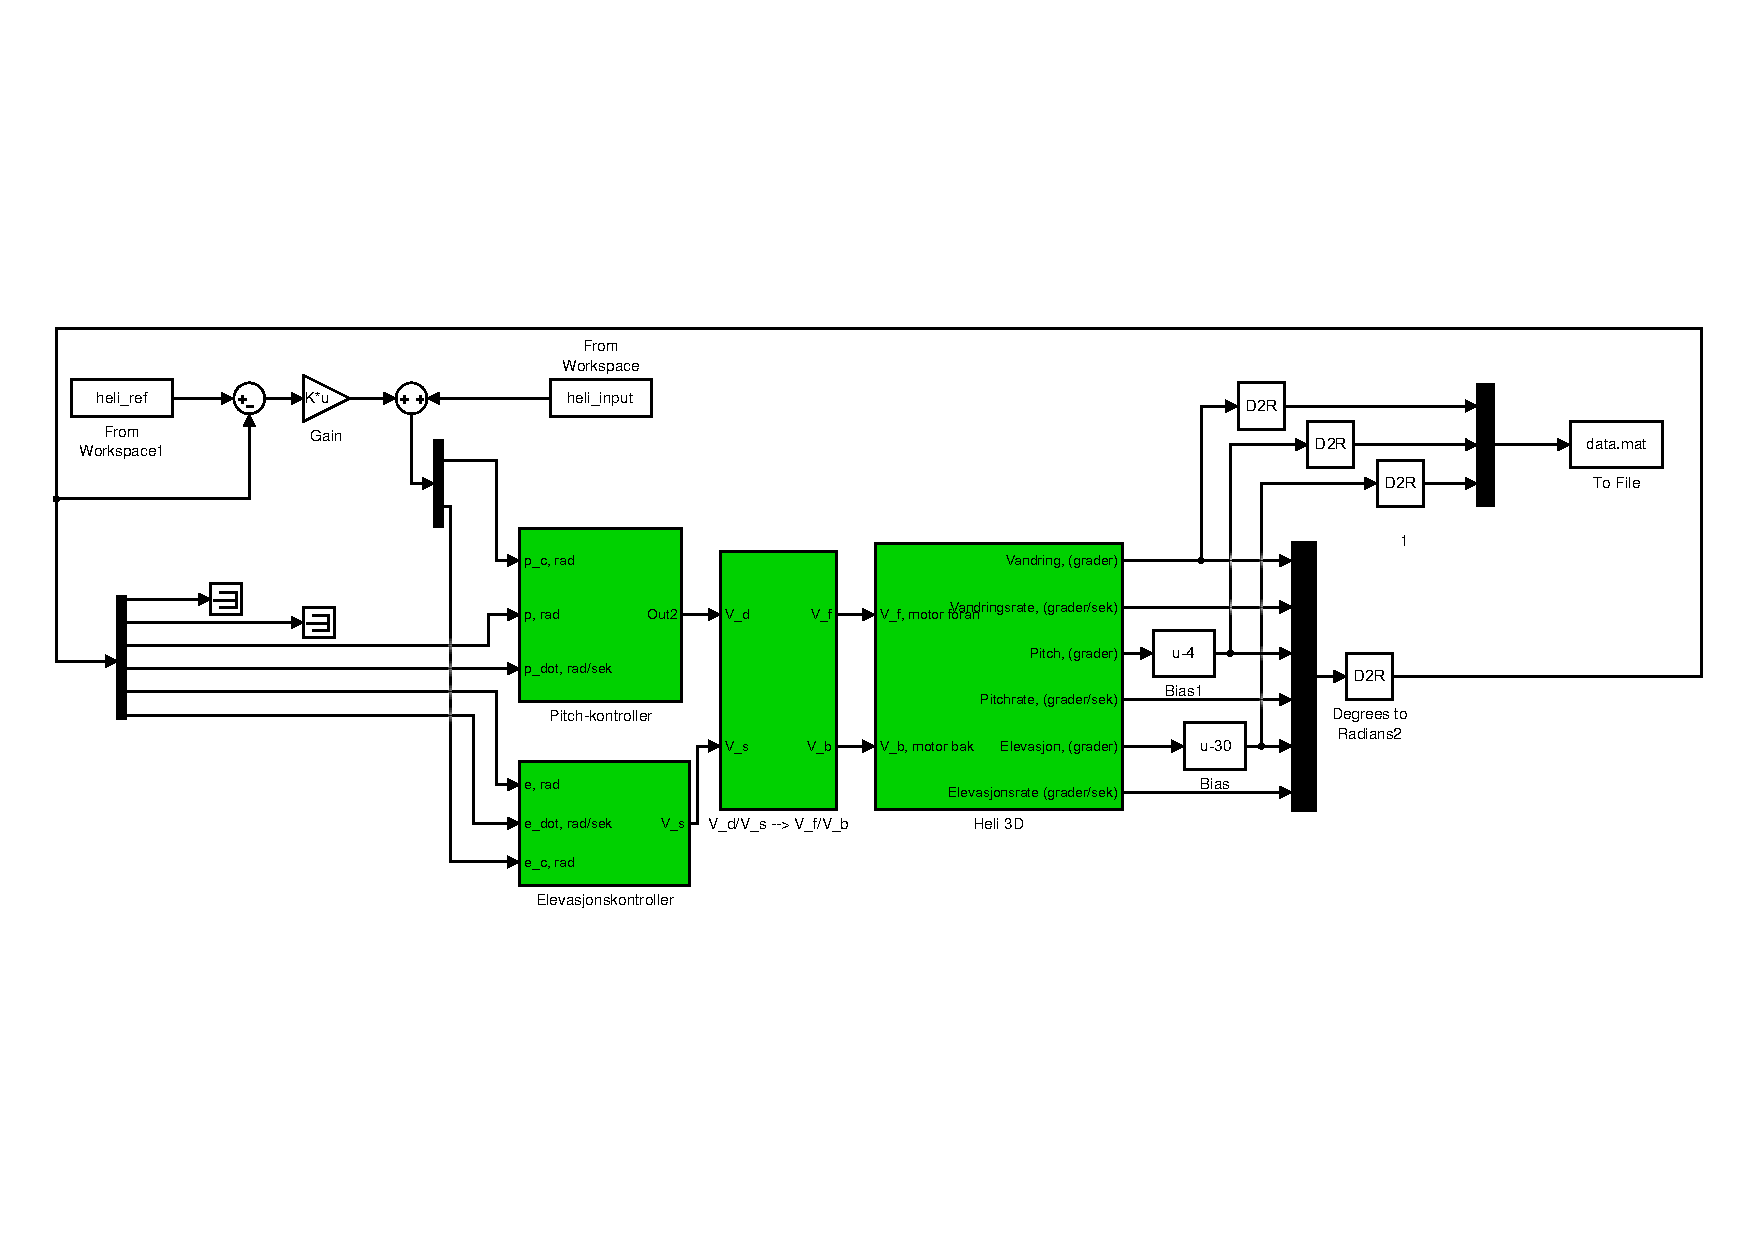
\includegraphics[width = 0.80\textwidth]{figures/4/simulink.pdf}
	\caption{Simulink model used in section \ref{text:problem4}.}
\end{figure}
